%!TEX root = ../main.tex

\section{Адаптация шага по времени}

\begin{frame}{Разностная схема}
\vspace{-3mm}
\begin{enumerate}
	\item $\; \Div_h \left( \epsilon[\phi] \nabla_h \hat{\Phi} \right) = - \rho_E \quad \leadsto \quad \hat{\Phi}$
	\item $\left[ \partt{\phi} \right]_h = m \cdot \left( -F'( \phi; \| \nabla_h \hat{\Phi} \|) + \cfrac{\Gamma}{2} \Delta_h \phi + \beta \Gamma l^2 \Div_h \left( \| \nabla_h \phi \|_2^2 \nabla_h \phi \right) \right)$
	\item $\left[ \partt{\rho} \right]_h = \Div_h \left( \sigma[\phi] \nabla_h \hat{\Phi} \right)$
	\item $\hat{\phi} = \phi + \tau \cdot \left[ \partt{\phi} \right]_h; \qquad \hat{\rho}_E = \rho_E + \tau \cdot \left[ \partt{\rho} \right]_h$
\end{enumerate}
\vspace{2mm}
\parind $\Pi = \sum h^3 \cdot \left( F(\phi; \| \nabla_h \Phi \|) + \cfrac{\Gamma}{4} \| \nabla_h \phi \|_2^2 + \cfrac{\beta}{4} \Gamma l^2 \| \nabla_h \phi \|_2^4 \right)$
\end{frame}


\begin{frame}{Проблемы}
\large
\begin{itemize}
	\setlength\itemsep{3mm}
	\item Нелинейная модель
	\item Сложная динамика с различным временным масштабом процессов
	\item Необходимость решать СЛАУ на каждом шаге
	\item Значительные ограничения на шаг по времени из-за параболичности оператора и нелинейности
\end{itemize}
\end{frame}


\begin{frame}{Адаптация по фазовому полю}
Работа \cite{ponomarev_adaptation}
\vspace{1mm}
\begin{block}{Формула расчета адаптивного шага}
	\[
		\tau^k = \max \left[ \taumin, \min \left( \taumax, \cfrac{\Tol}{\left\| [\partflt{\phi}]_h \right\|_C} \right) \right]
	\]
\end{block}
\vspace{1mm}
\parind Идея метода:
\[
	\| \hat{\phi} - \phi \|_C = \tau^k \cdot \left\| \left[ \partt{\phi} \right]_h \right\|_C = \cfrac{\Tol}{\left\| [\partflt{\phi}]_h \right\|_C} \cdot \left\| \left[ \partt{\phi} \right]_h \right\|_C \approx \Tol
\]
\parind Предложен в статье \cite{li_time_step}
\end{frame}


\begin{frame}{Граничные условия}
\centering
Кубический образец диэлектрика, зажатый между двумя проводящими пластинами. \\[5mm]
\begin{tabular}{{%
    >{\centering\arraybackslash}m{60mm}%
    >{\centering\arraybackslash}m{60mm}%
}}
	Обкладки сверху и снизу: & Боковая граница $\partial \Omega$: \\[1mm]
	\cellcentered{12mm}{\centering $\Phi|_{z = 0} = \Phi^+; \; \Phi|_{z = L} = \Phi^-$} &
	\cellcentered{12mm}{\centering $\partvn{\Phi}\bigg|_{\partial \Omega} = 0$} \\
	\cellcentered{12mm}{\centering $\cfrac{\partial \phi}{\partial z}\bigg|_{z = 0} = \cfrac{\partial \phi}{\partial z}\bigg|_{z = L} = 0$} &
	\cellcentered{12mm}{\centering $\phi|_{\partial \Omega} = 1$}
\end{tabular}
\end{frame}


\begin{frame}{Расчет №1: <<иголка>>}
\vspace{-5mm}
\begin{figure}
	\subfloat[Начальное условие]{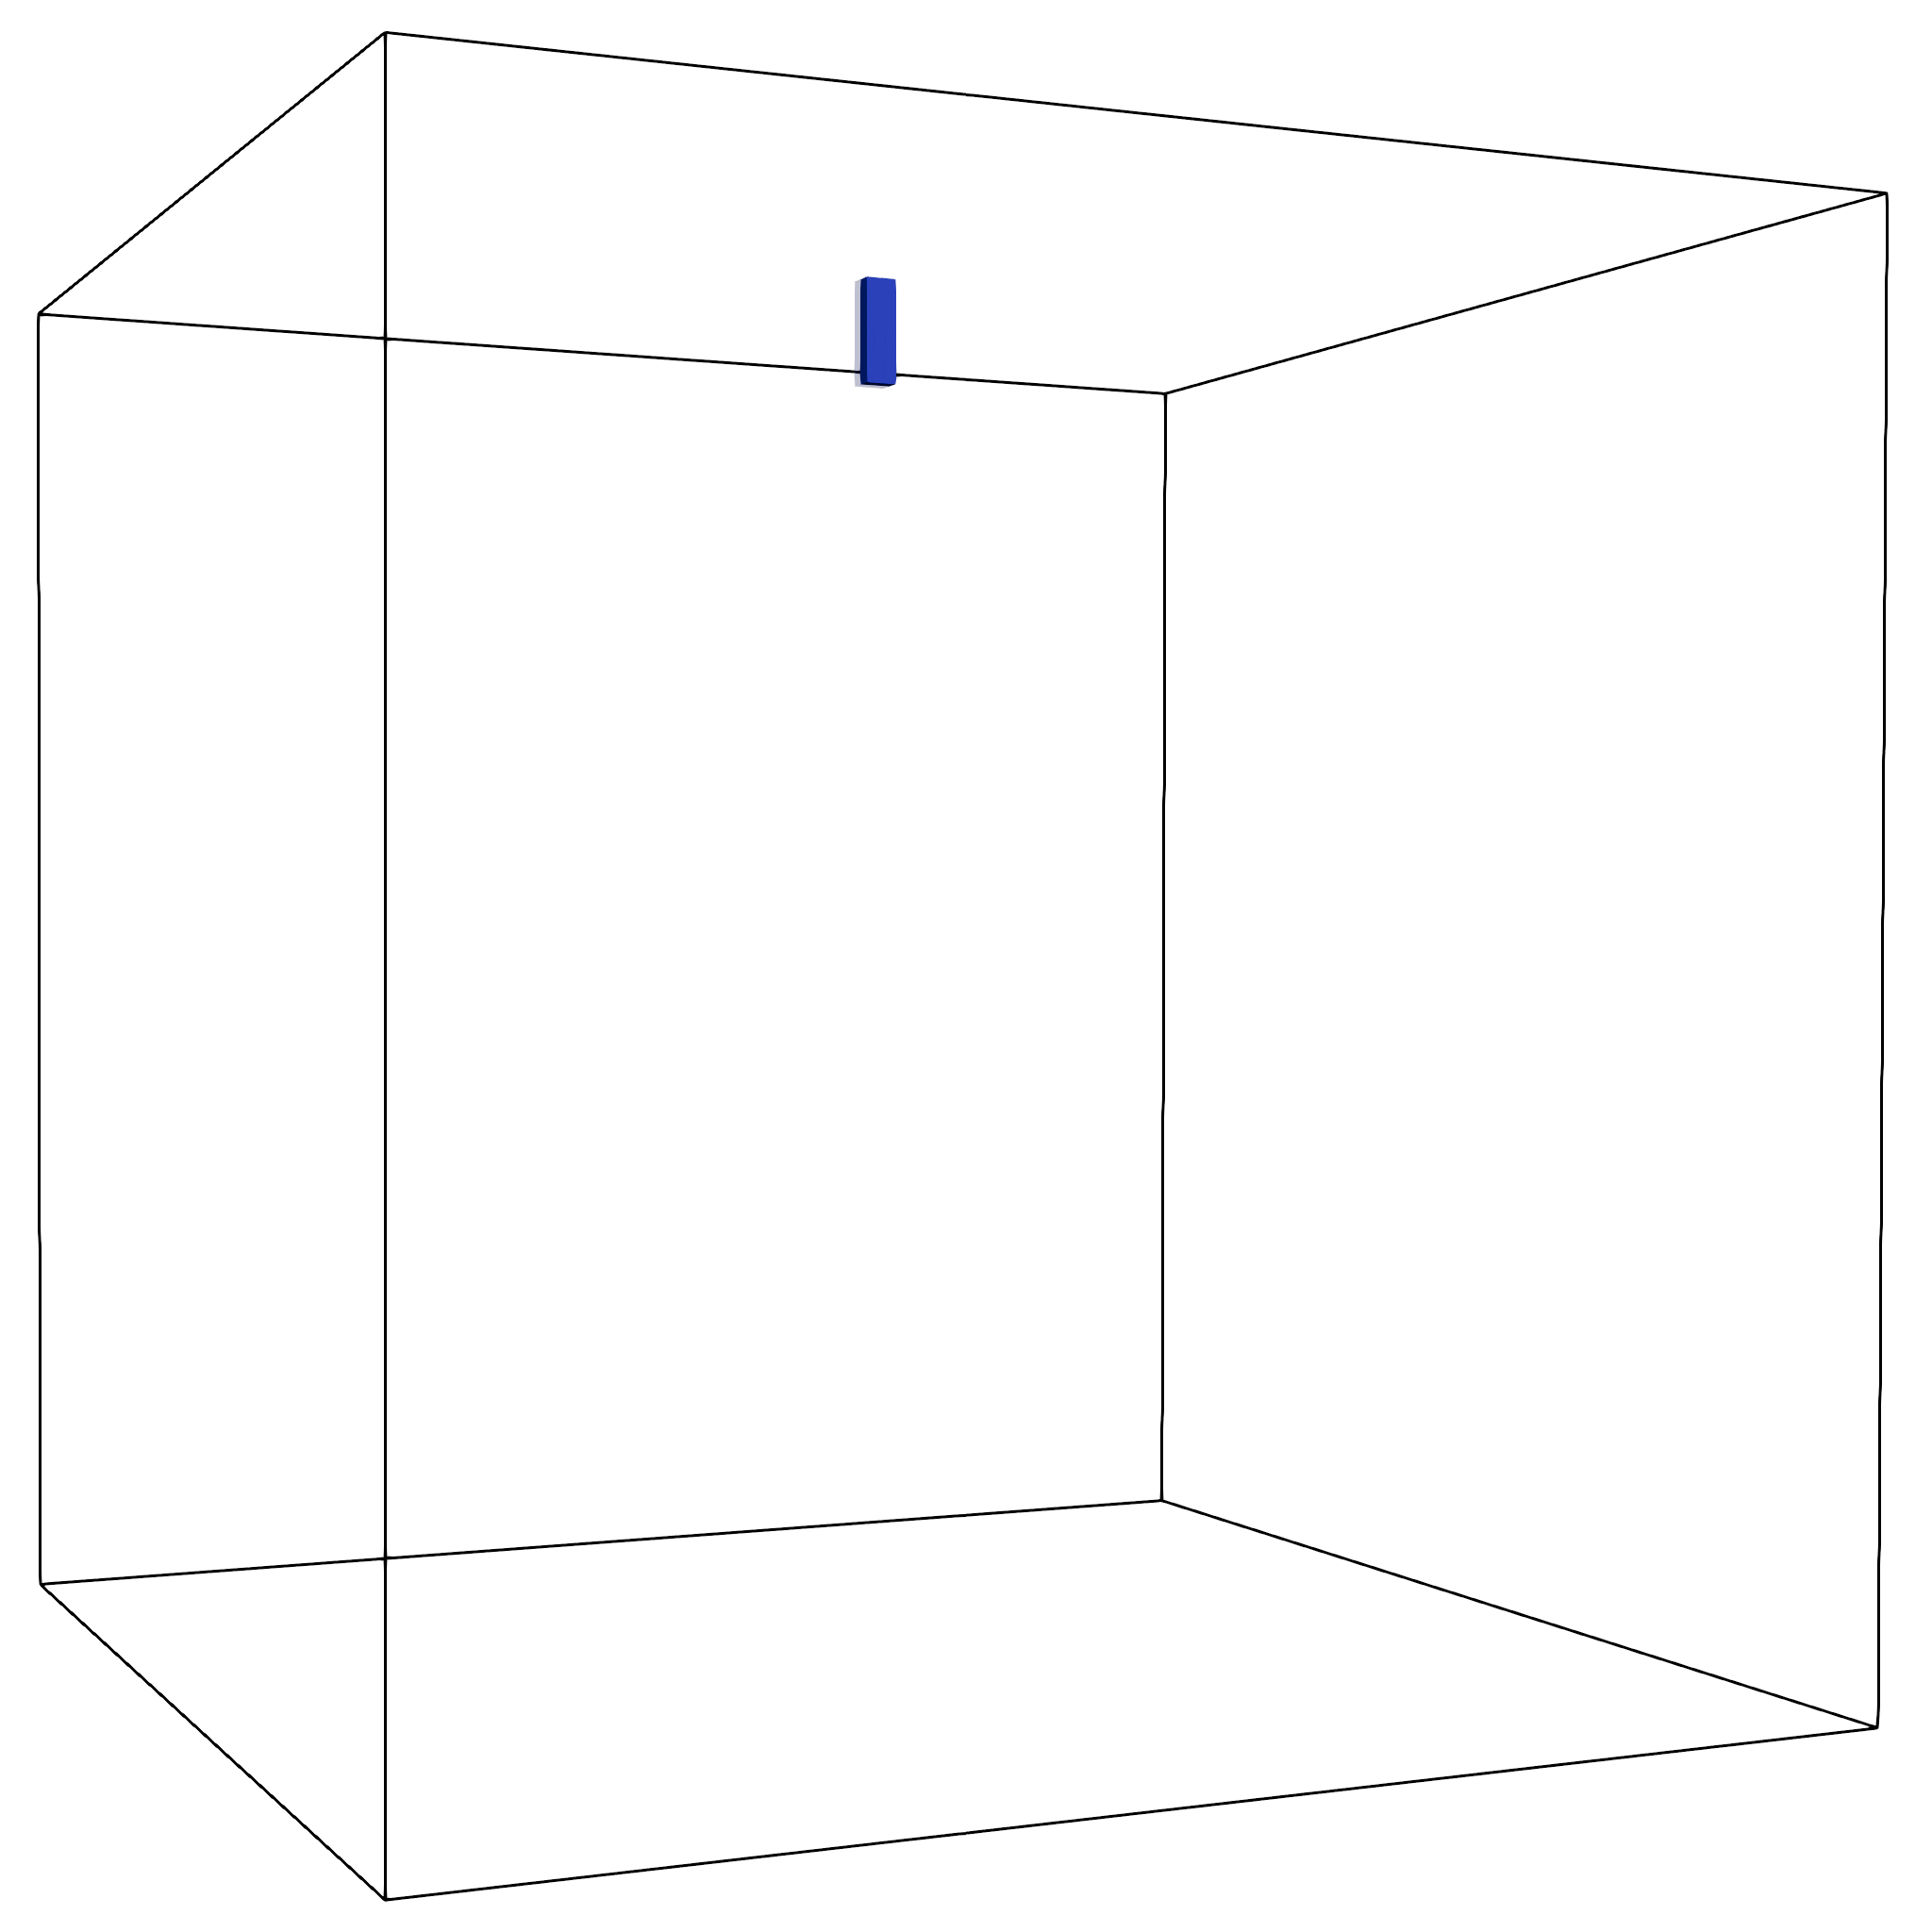
\includegraphics[width=0.333\textwidth]{figures/needle_result_1.png}}
	\subfloat[Рост канала]{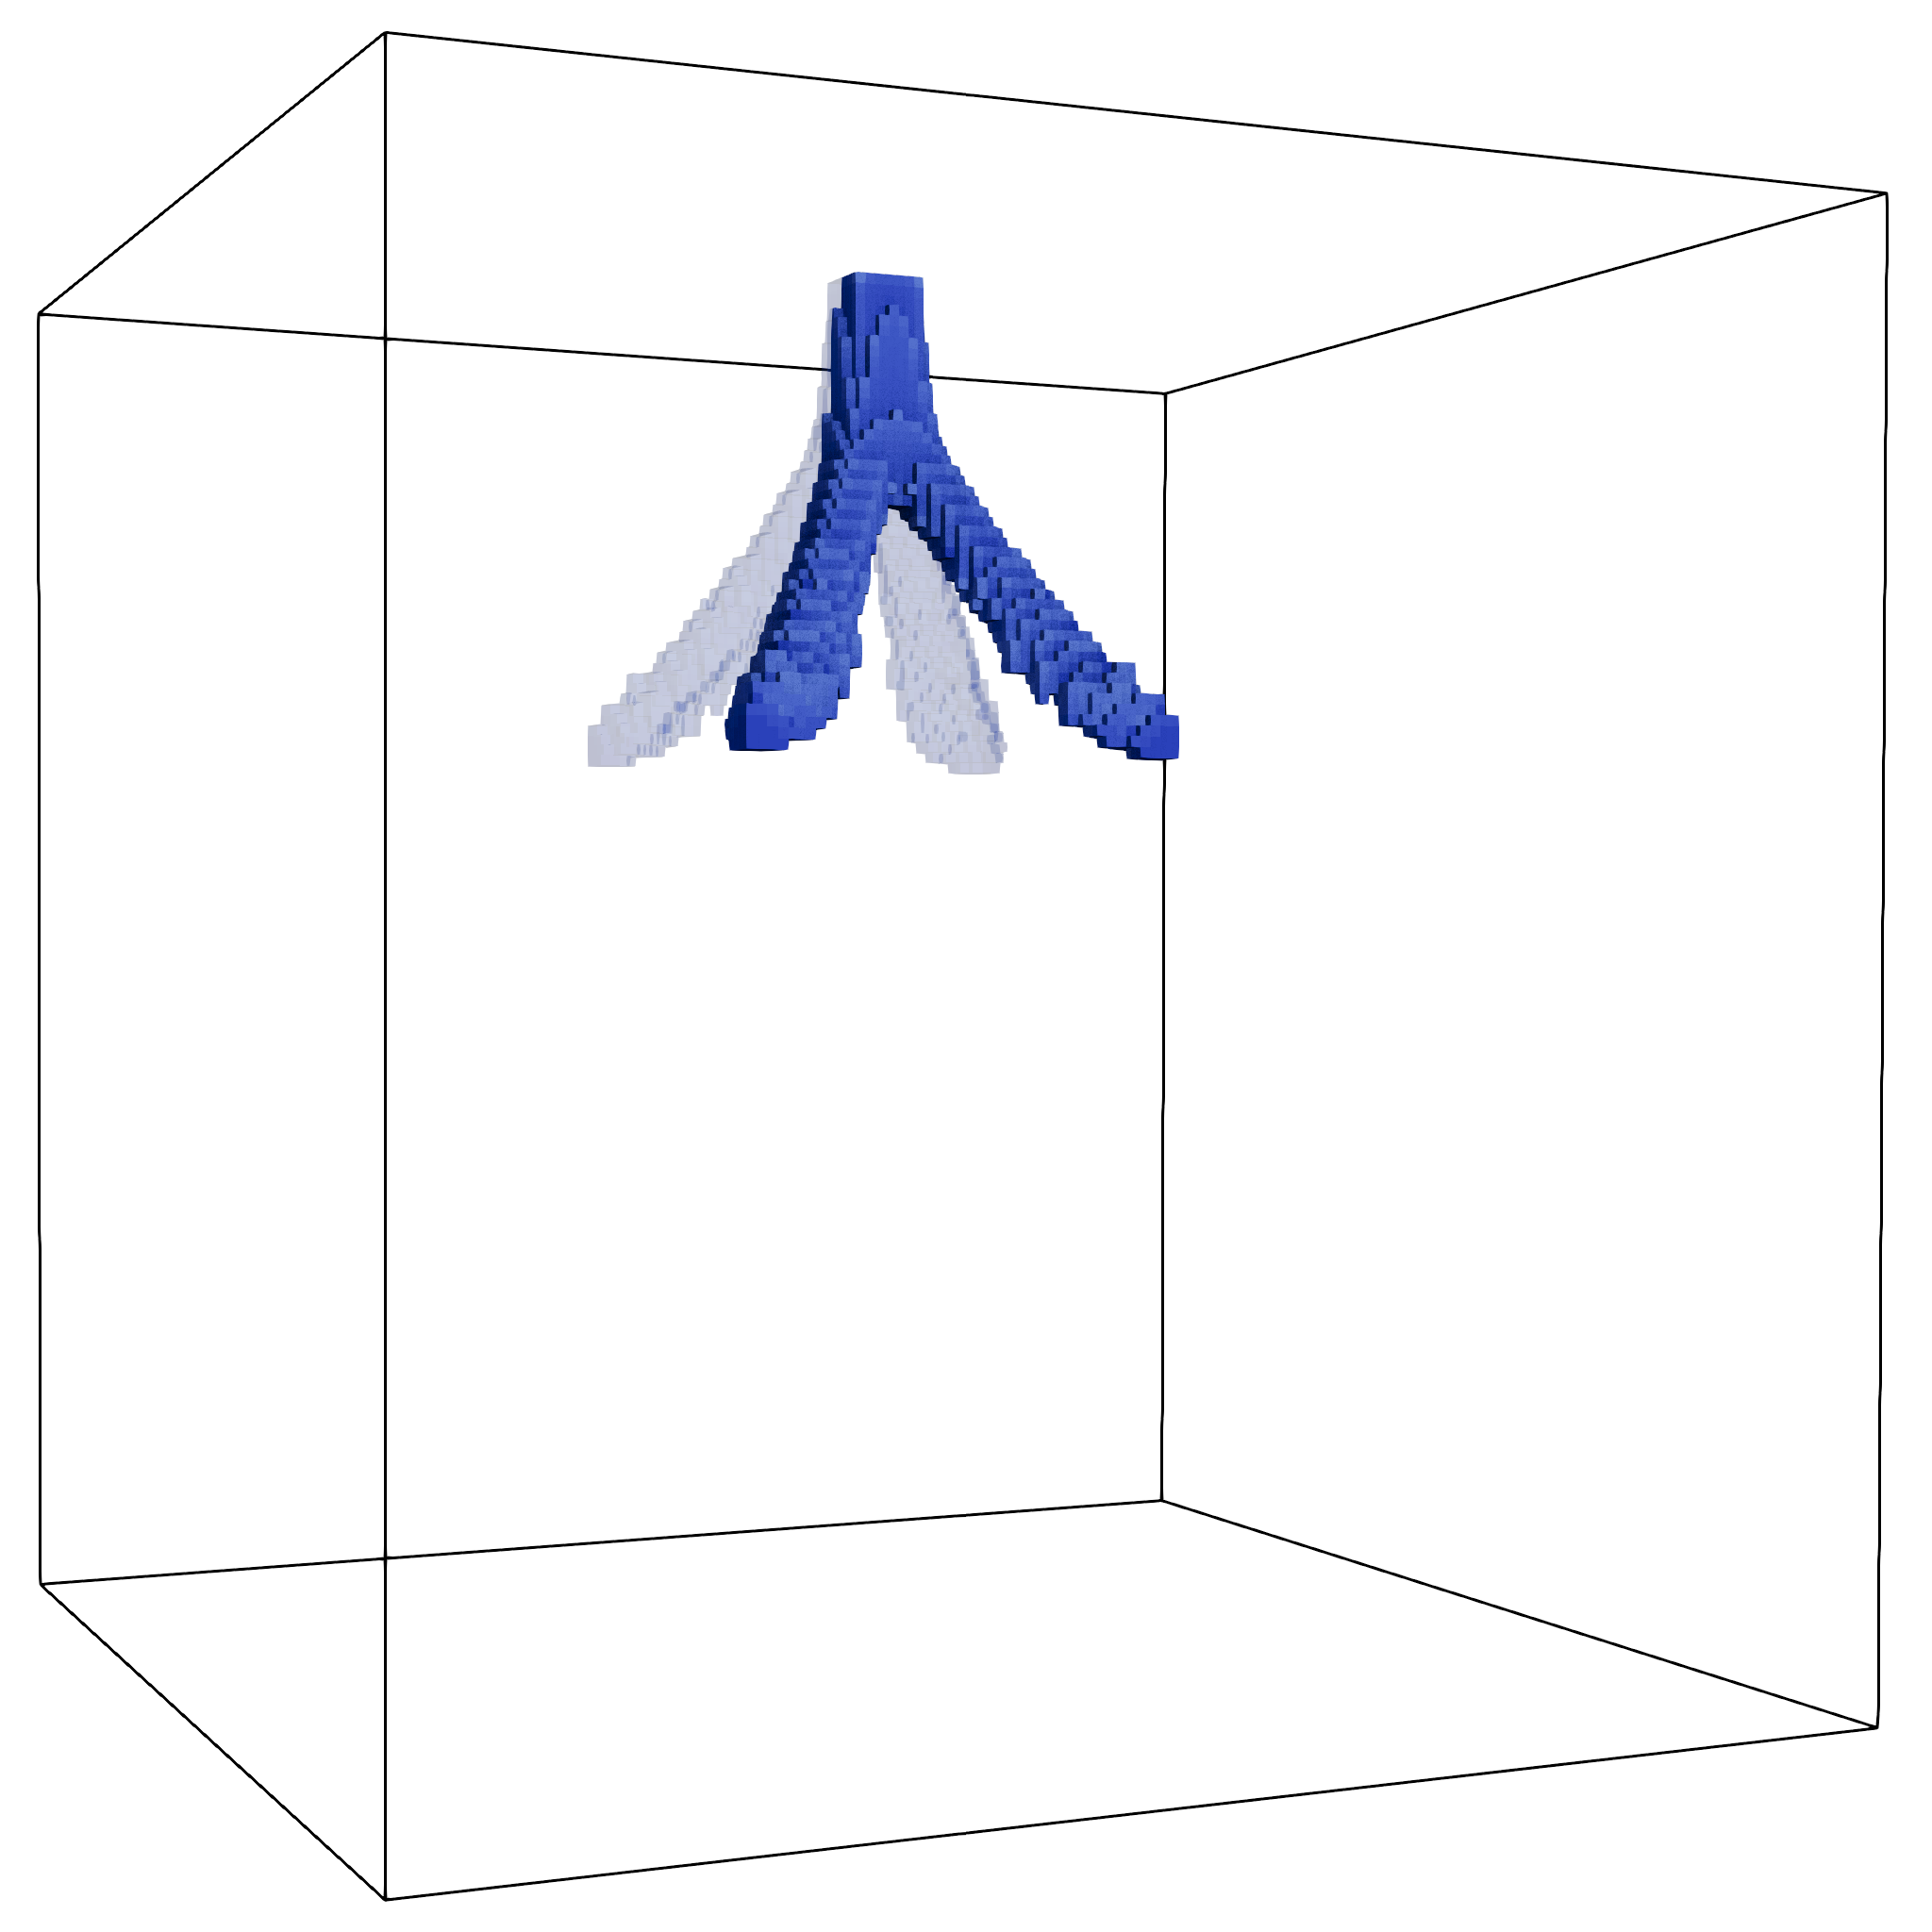
\includegraphics[width=0.333\textwidth]{figures/needle_result_2.png}}
	\subfloat[Перед пробоем <<насквозь>>]{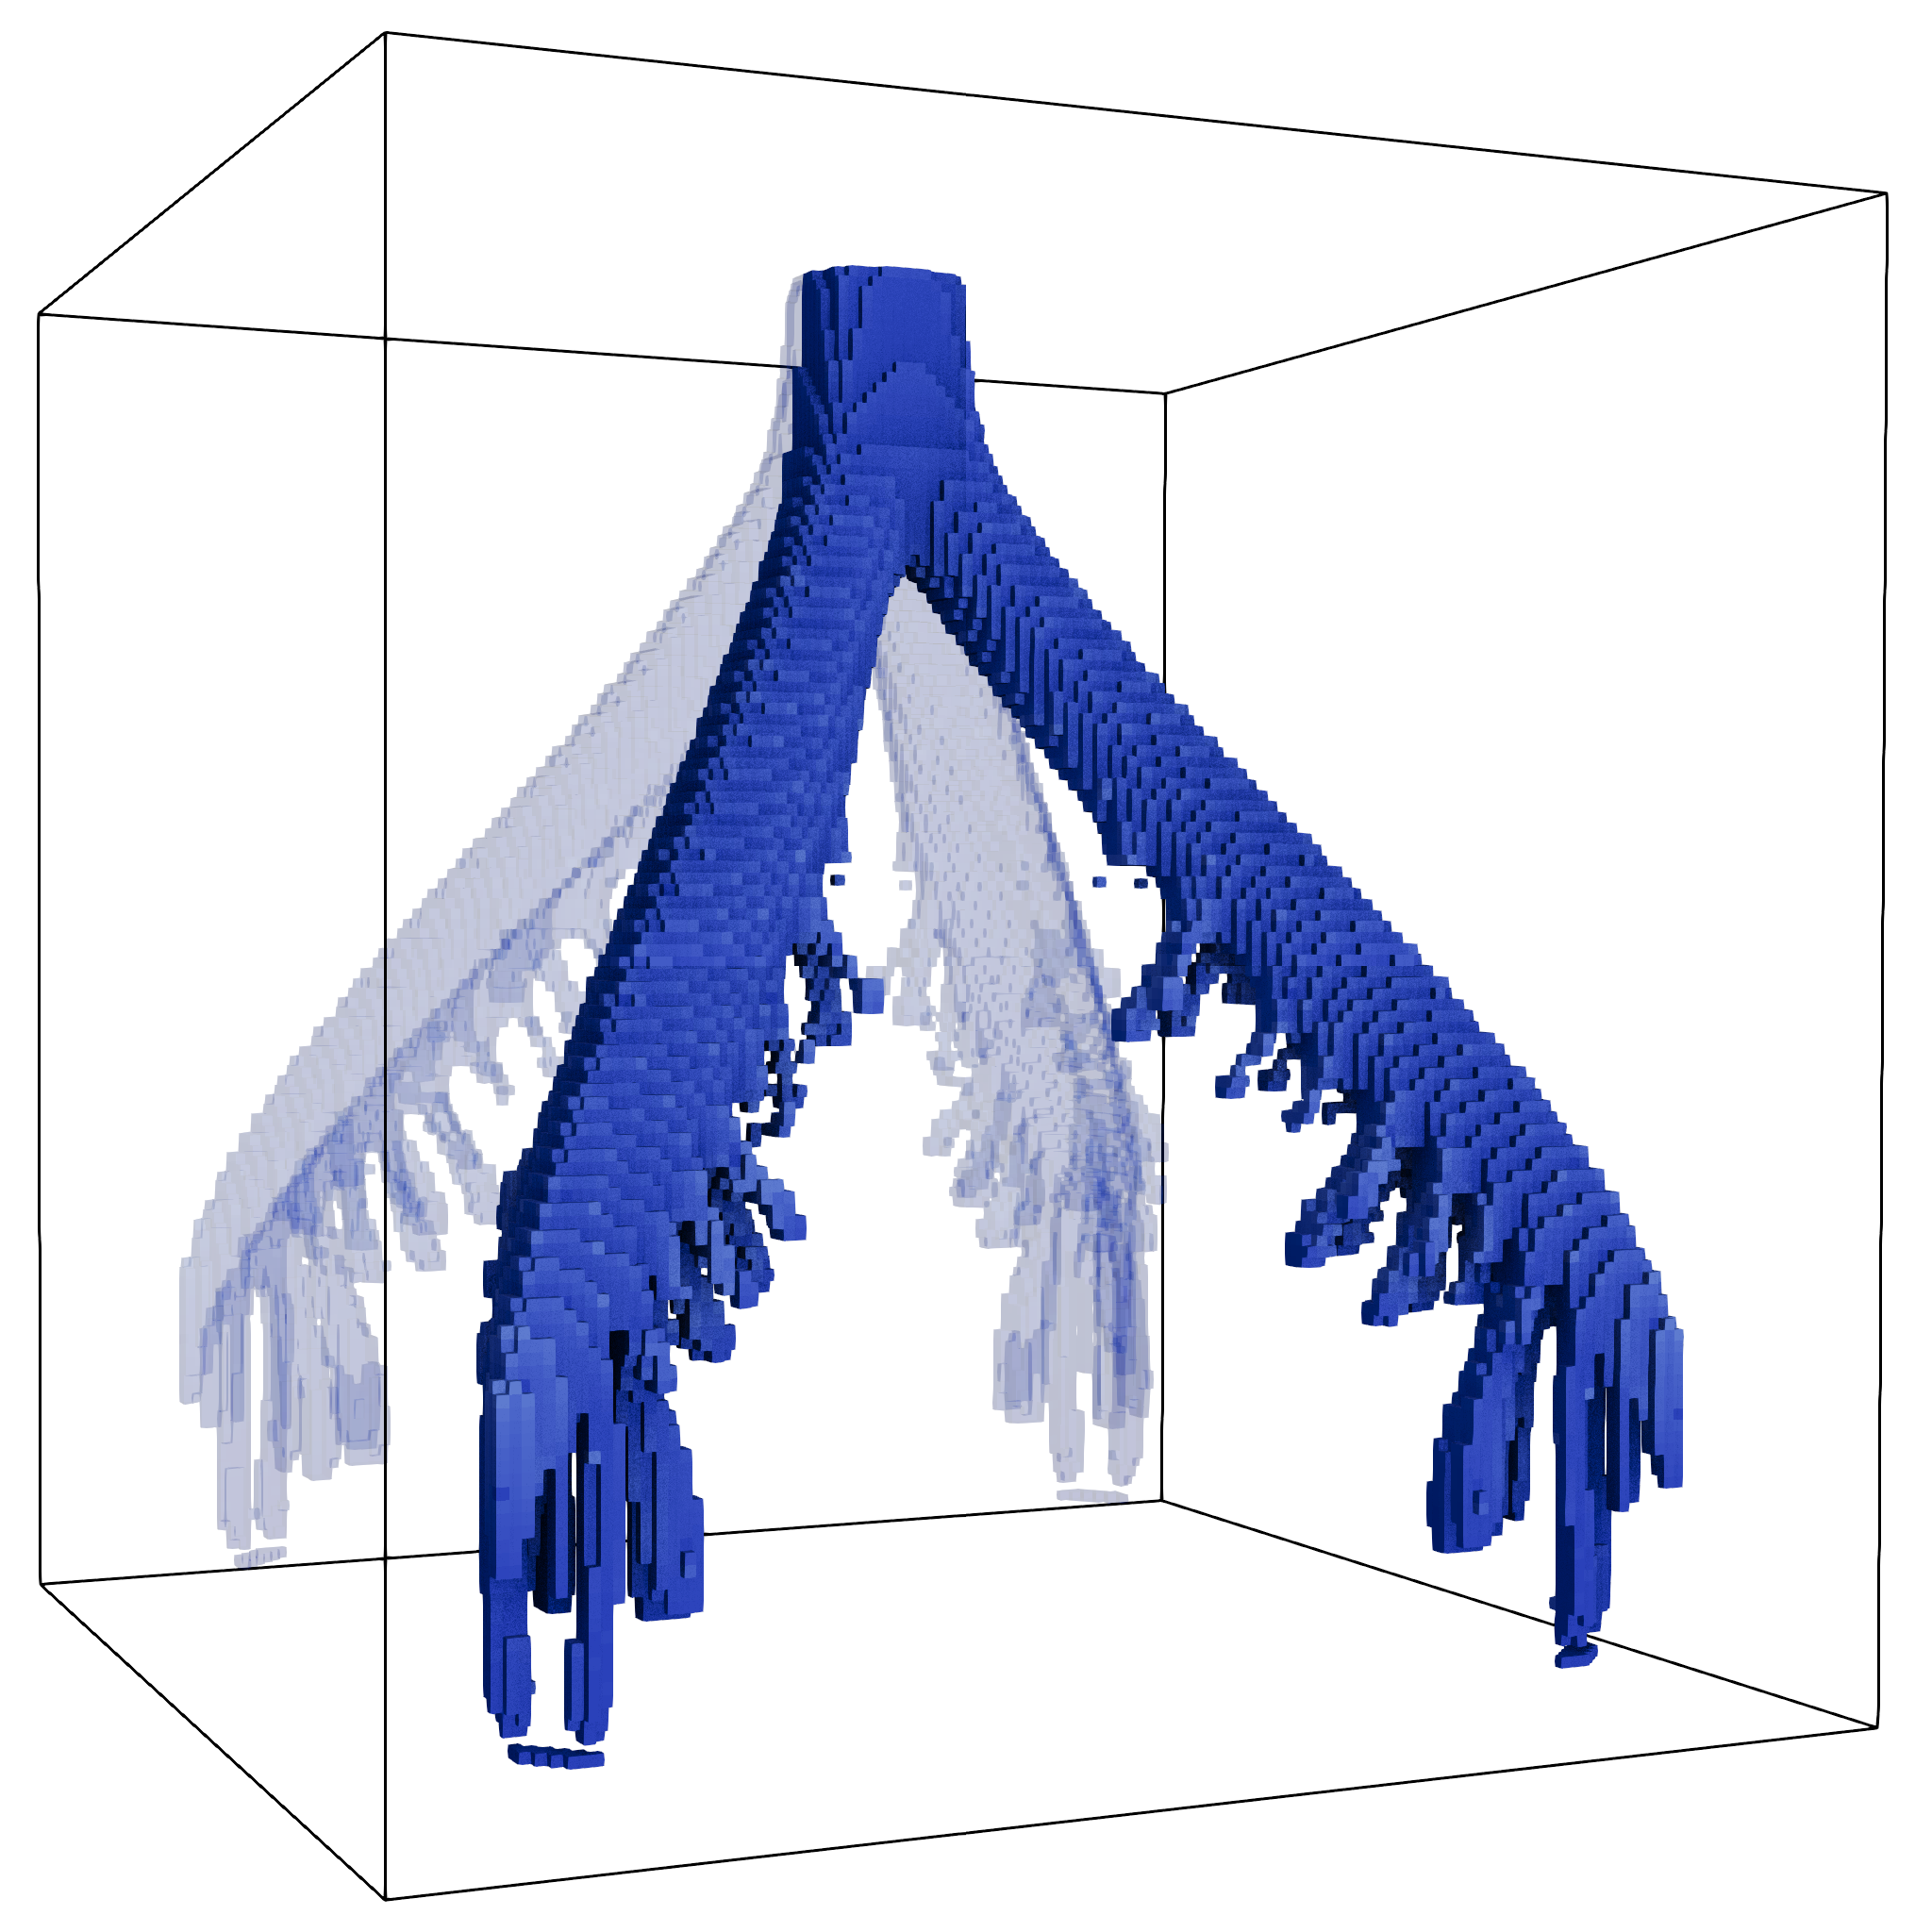
\includegraphics[width=0.333\textwidth]{figures/needle_result_3.png}}
\end{figure}
\vspace{-7mm}
\begin{minipage}[l]{0.93\textwidth}
\begin{align*}
	N_h &= 129 & T &\approx 7 \cdot 10^{-7} & \taumin &= 10^{-12} & 56 \text{ MPI-процессов} \\
	N_t &= 51000 & \Tol &= 10^{-2} & \taumax &= 10^{-7} &
\end{align*}
\end{minipage}
\end{frame}


\begin{frame}{Расчет №1: <<иголка>>}
\vspace{-2mm}
\begin{figure}
	\captionsetup[subfigure]{labelformat=empty}
	\subfloat[]{
\includegraphics[width=0.49\textwidth]{figures/needle_phi_mean.png}}
	\hfill
	\subfloat[]{
\includegraphics[width=0.49\textwidth]{figures/needle_energy.png}}
\end{figure}
\end{frame}


\begin{frame}{Расчет №2: случайные возмущения}
\vspace{-5mm}
\begin{figure}
	\subfloat[Зародыши каналов]{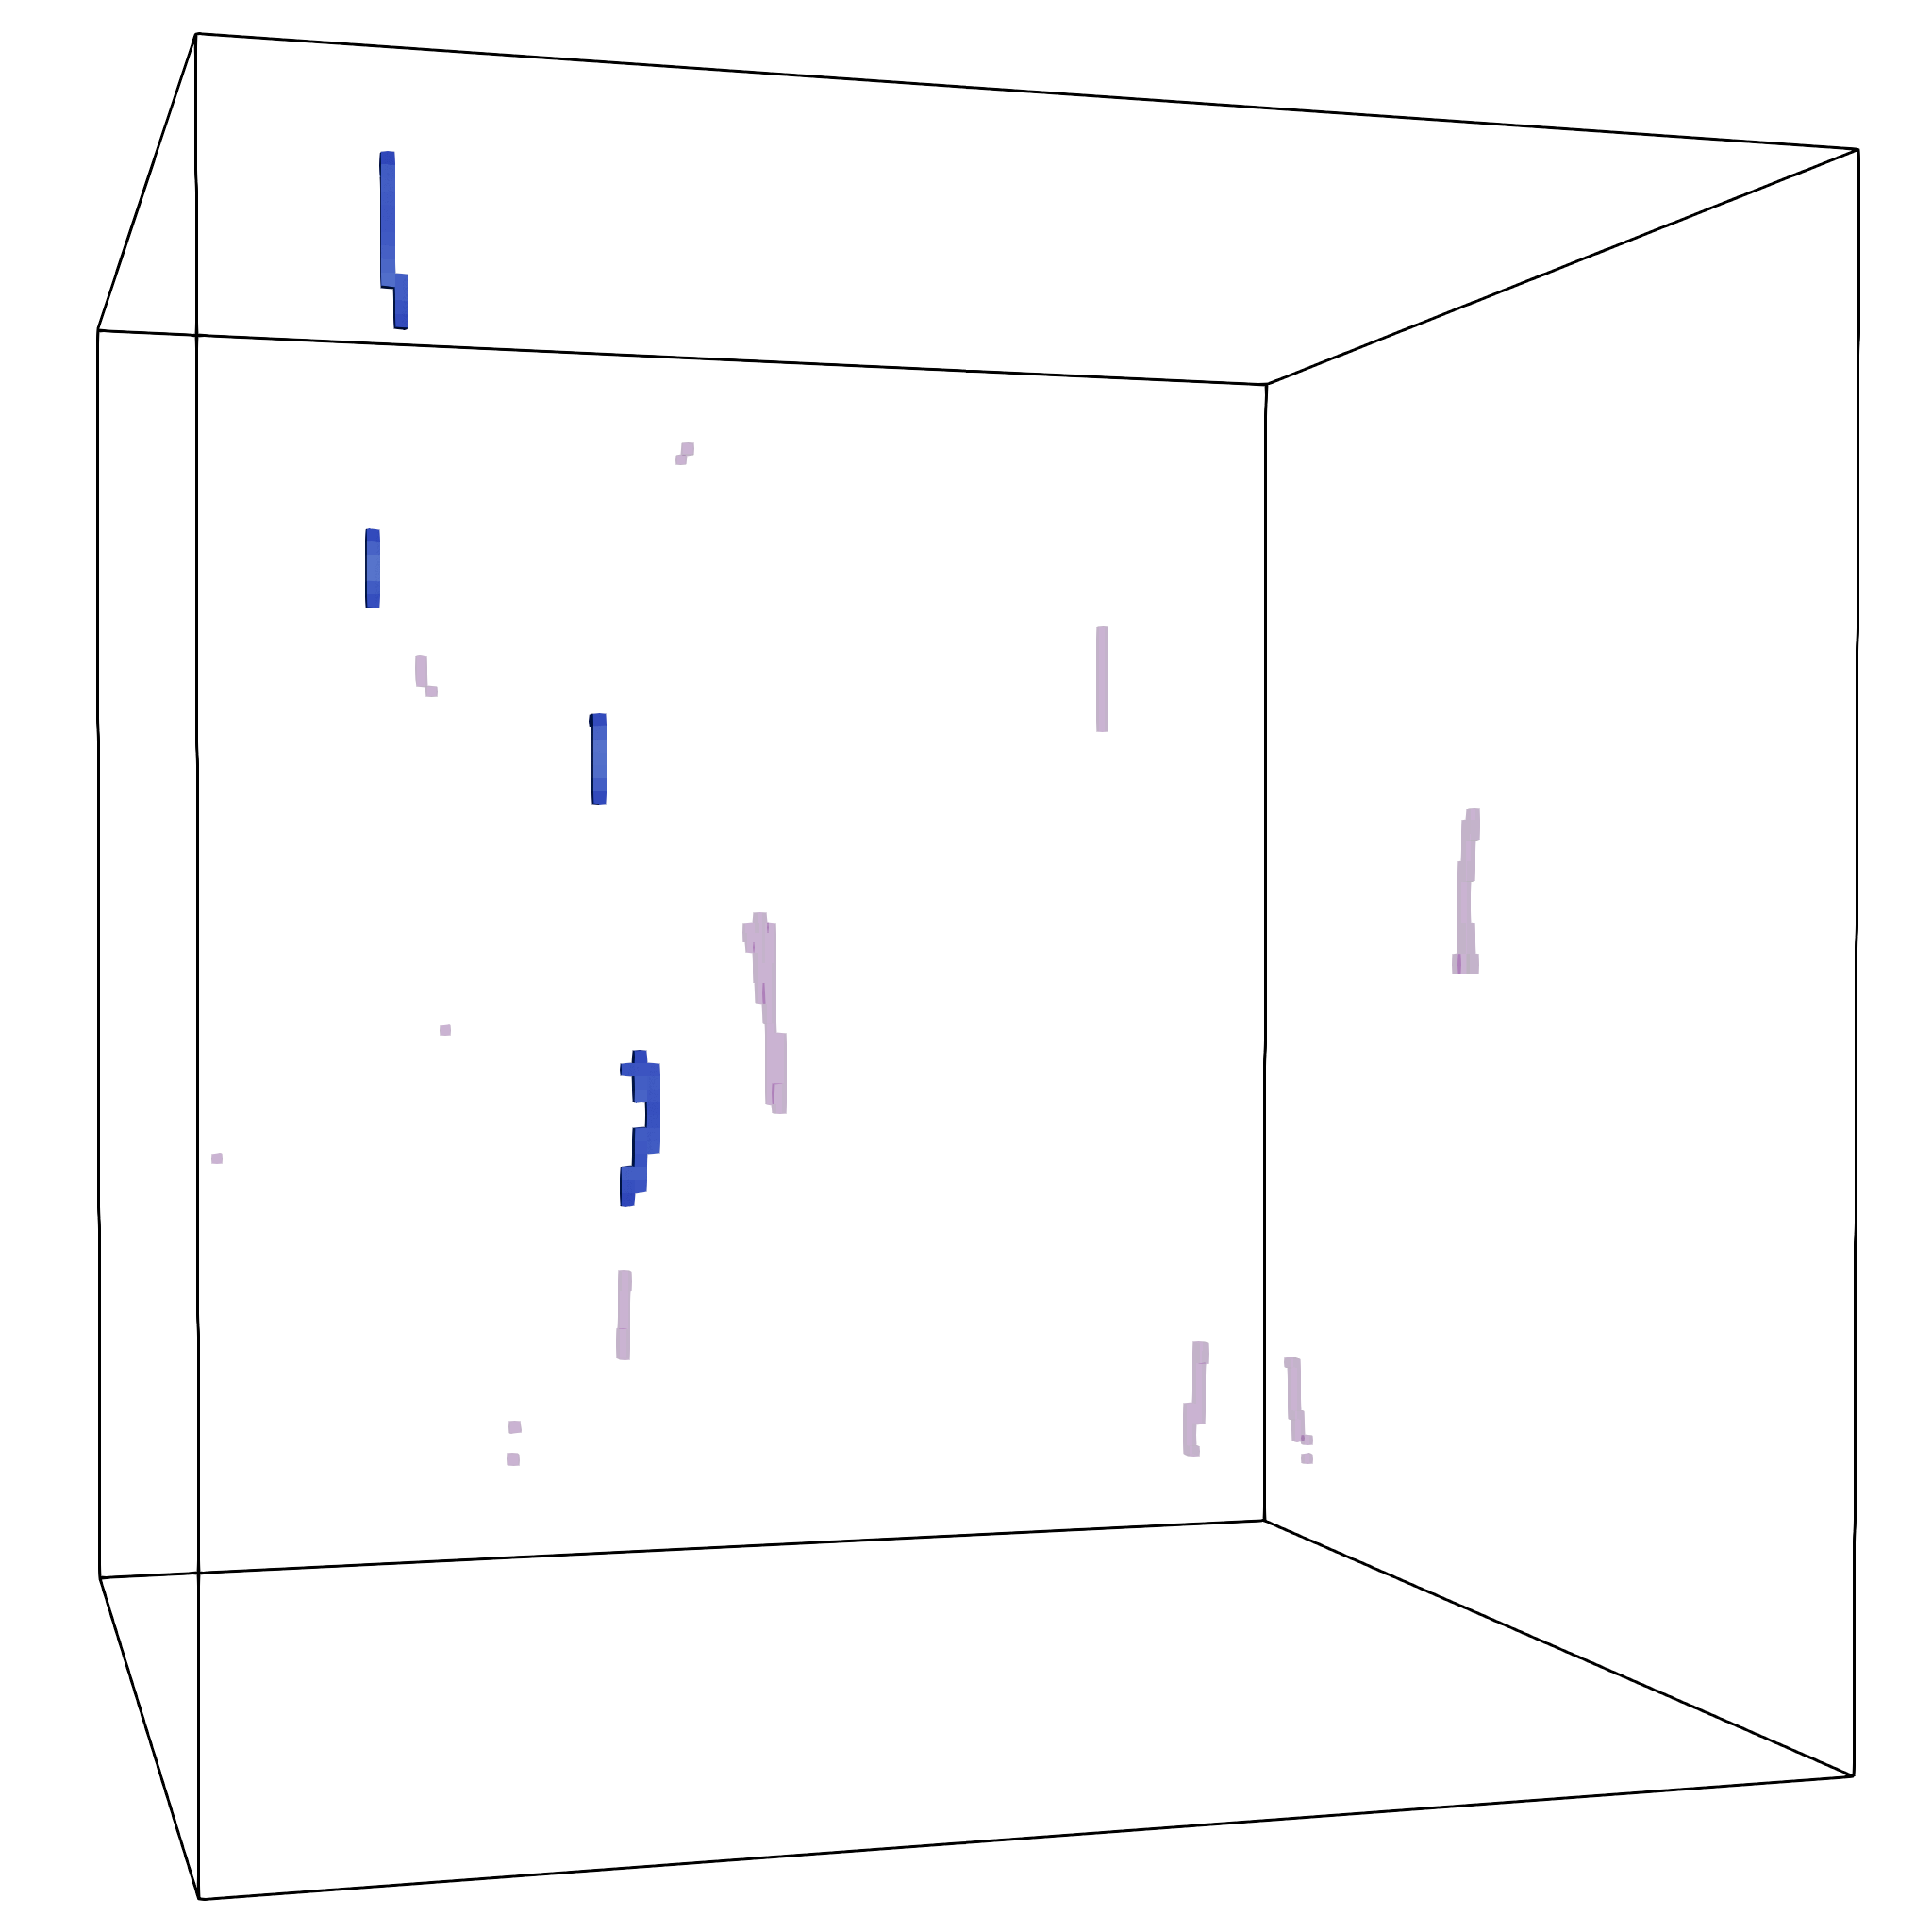
\includegraphics[width=0.333\textwidth]{figures/disturbance_result_1.png}}
	\subfloat[Рост и слияние]{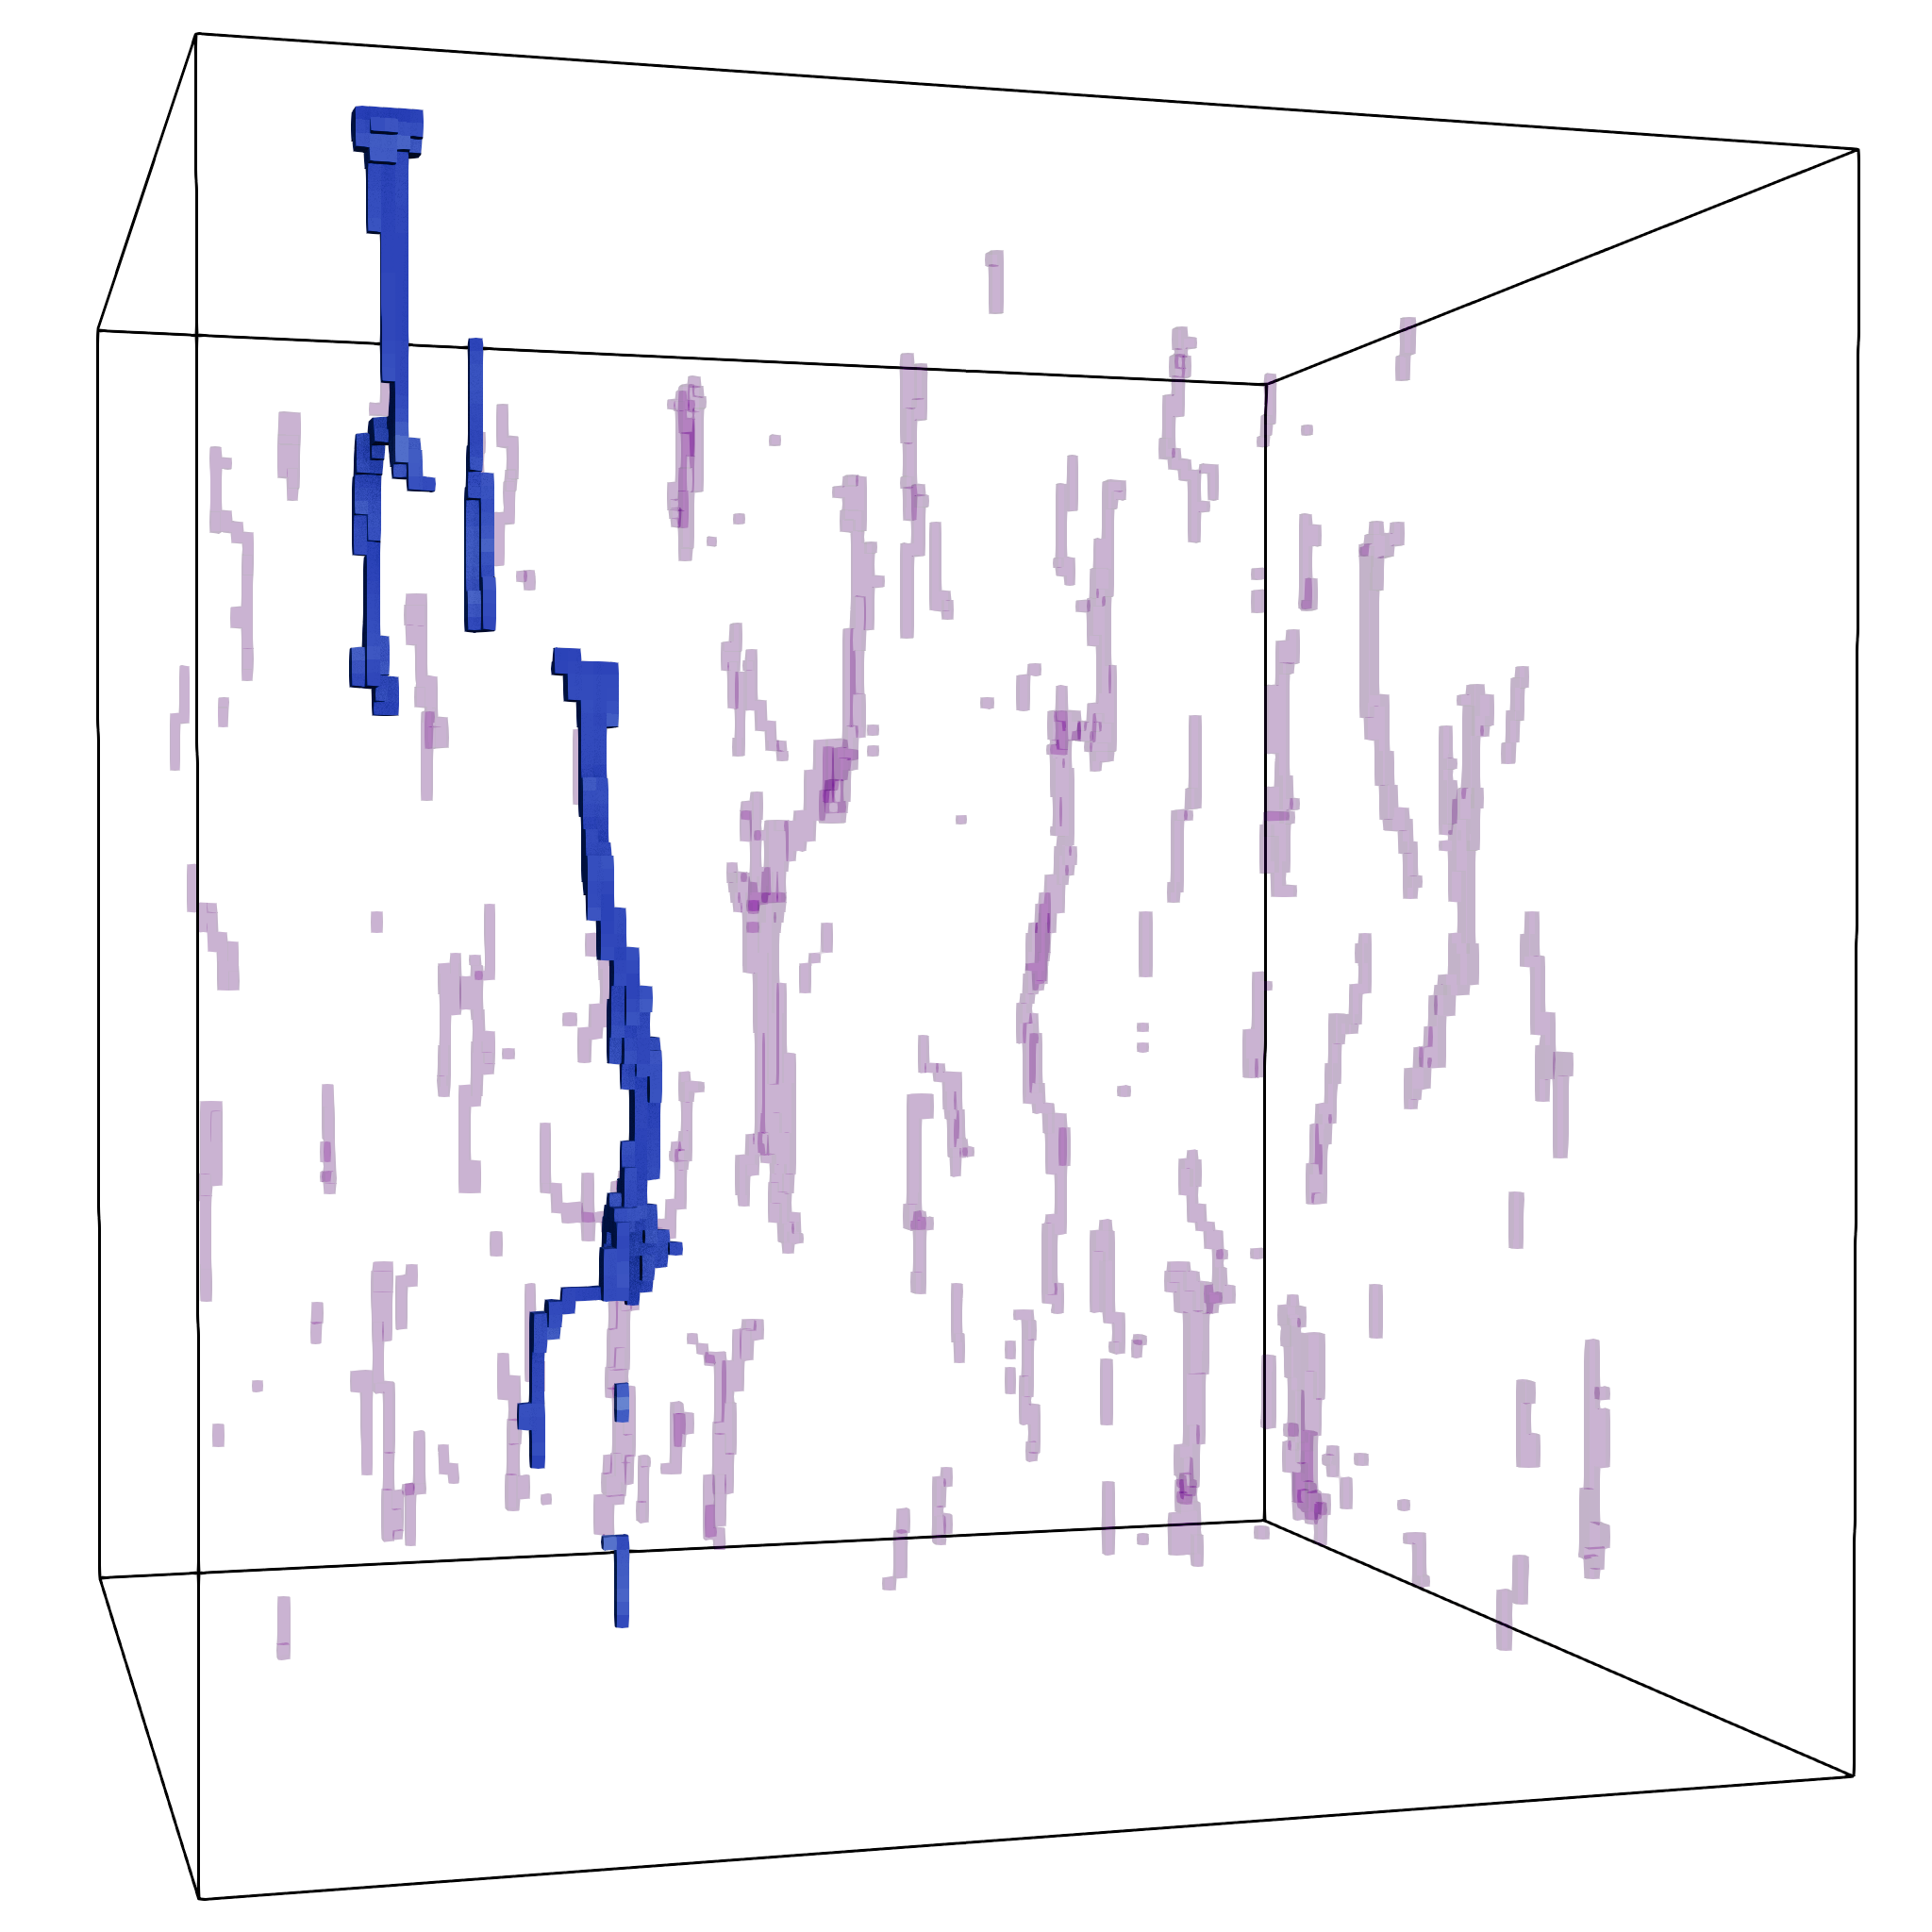
\includegraphics[width=0.333\textwidth]{figures/disturbance_result_2.png}}
	\subfloat[Пробой <<насквозь>>]{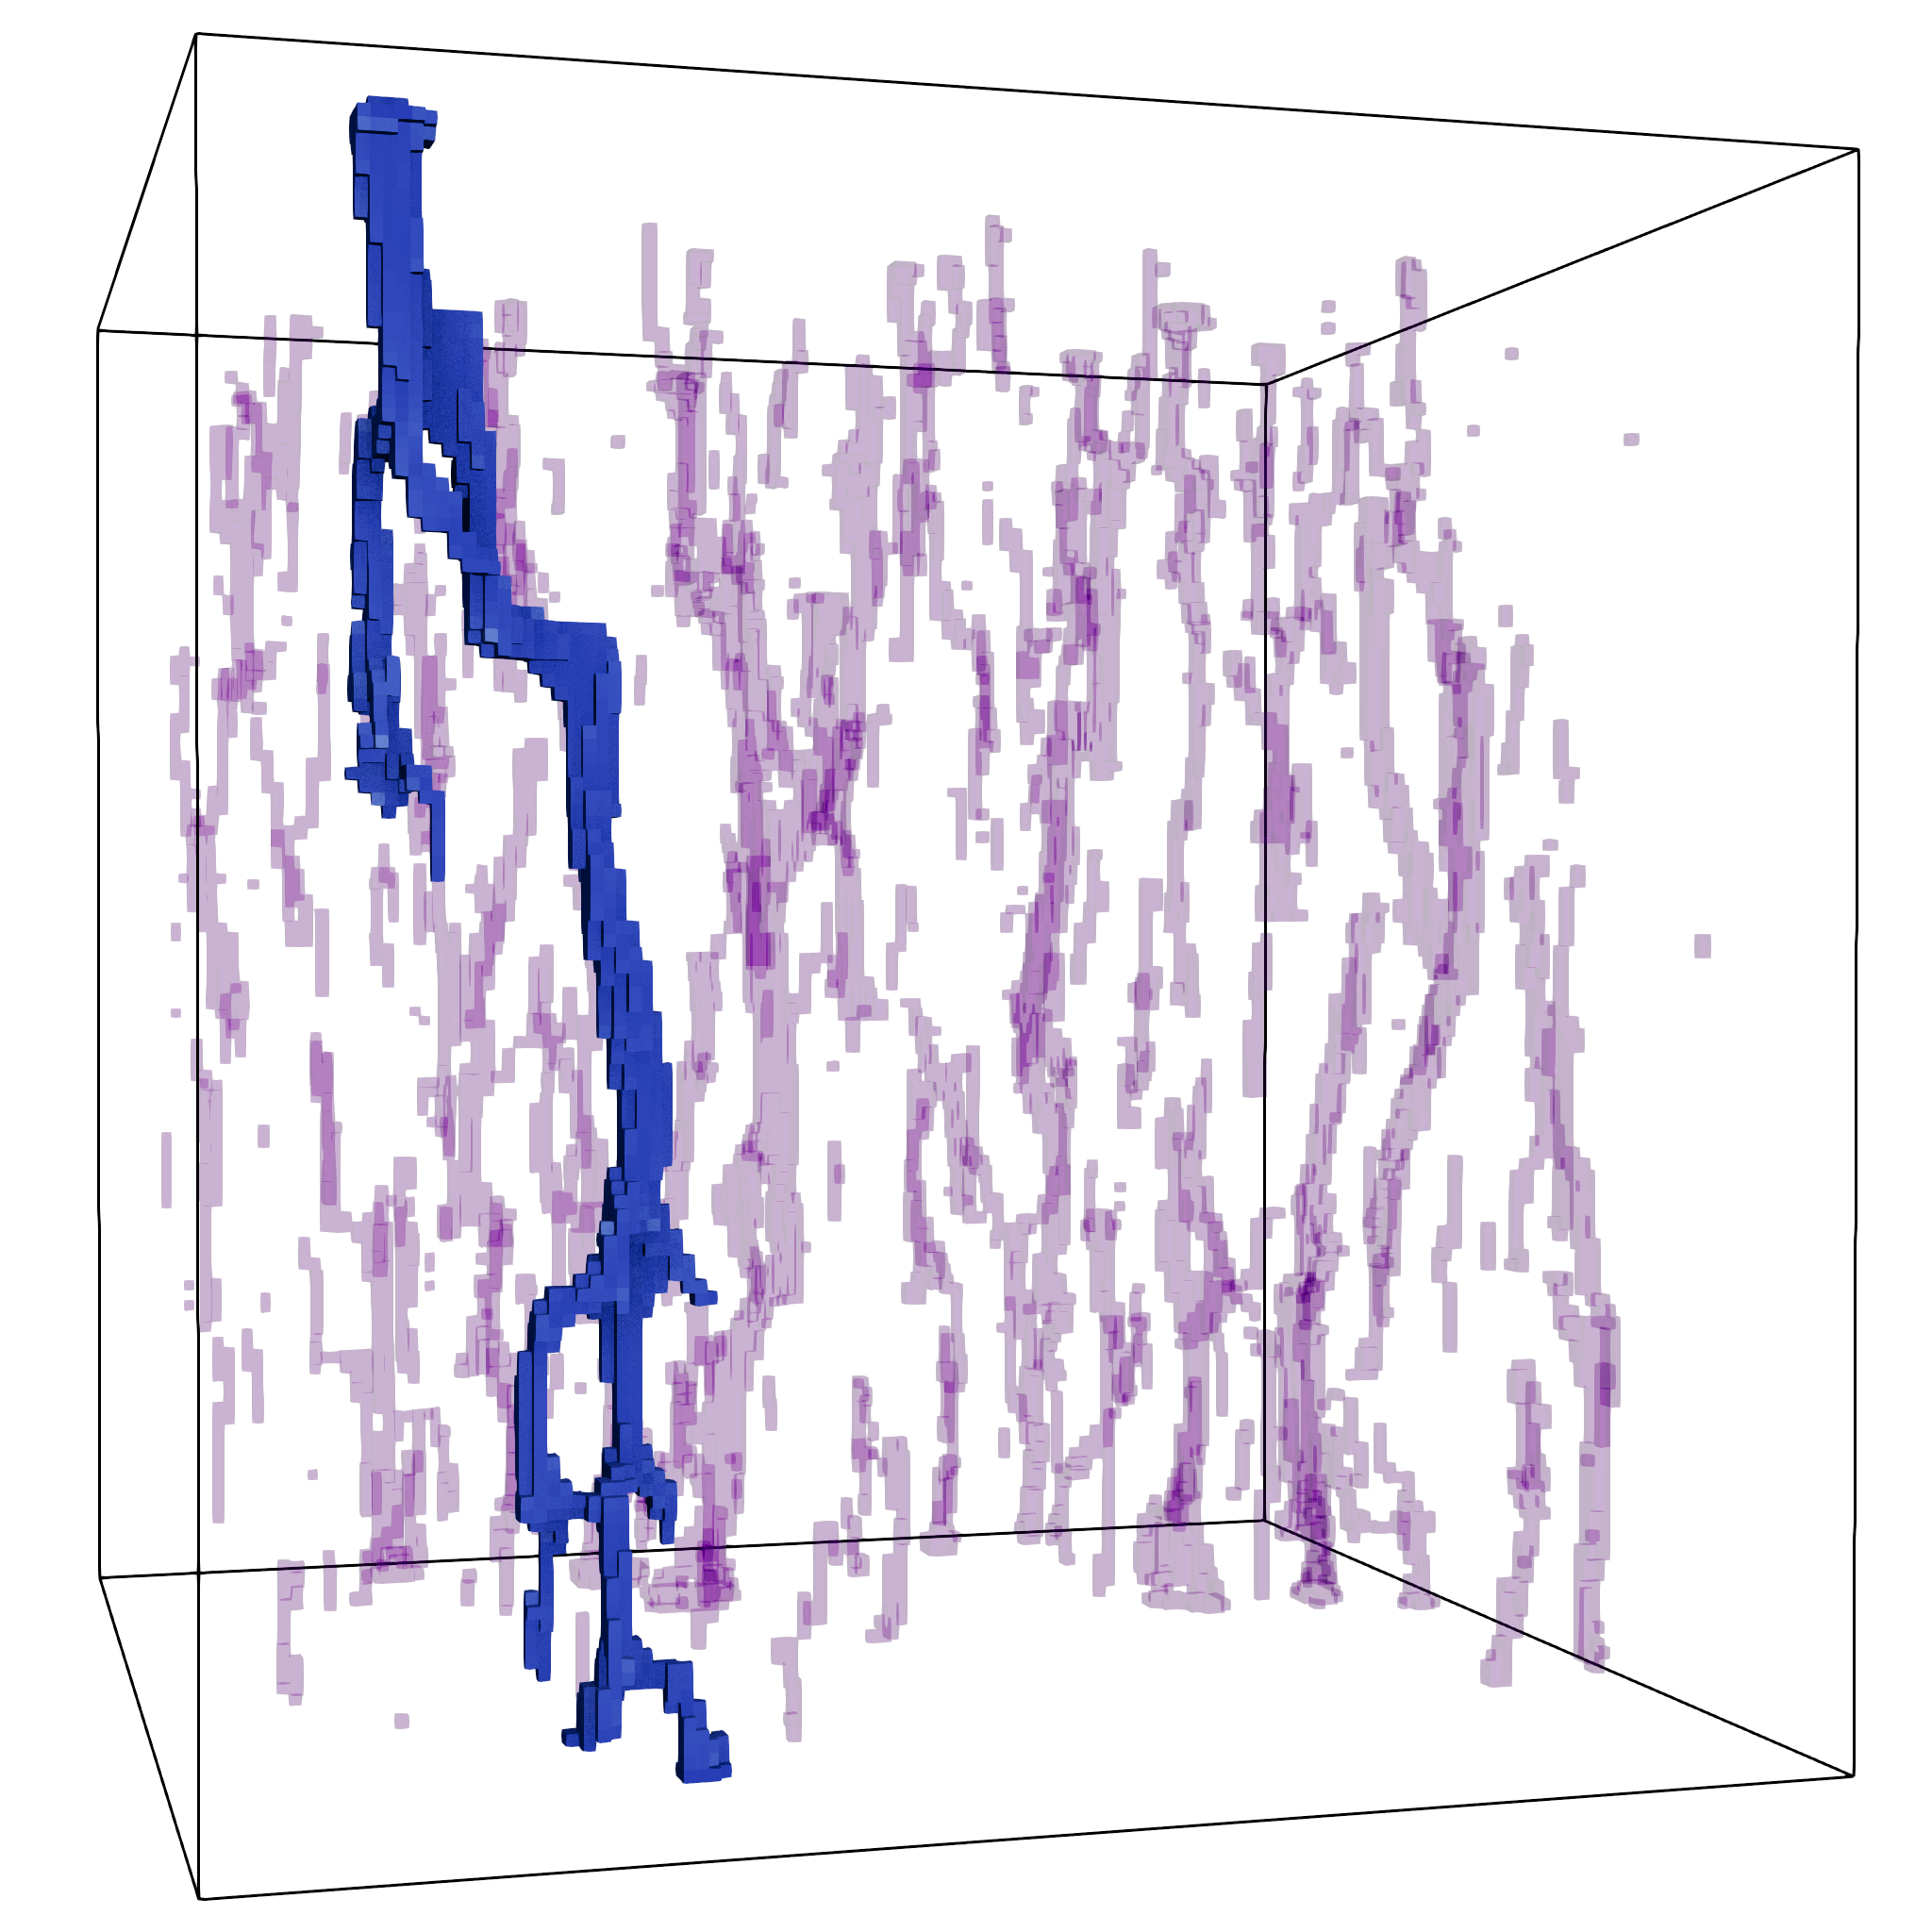
\includegraphics[width=0.333\textwidth]{figures/disturbance_result_3.png}}
\end{figure}
\vspace{-7mm}
\begin{minipage}[l]{0.93\textwidth}
\begin{align*}
	N_h &= 129 & T &\approx 1.7 \cdot 10^{-6} & \taumin &= 10^{-12} & 56 \text{ MPI-процессов} \\
	N_t &= 22000 & \Tol &= 10^{-2} & \taumax &= 10^{-7} &
\end{align*}
\end{minipage}
\end{frame}


\begin{frame}{Расчет №2: случайные возмущения}
\vspace{-2mm}
\begin{figure}
	\captionsetup[subfigure]{labelformat=empty}
	\subfloat[]{
\includegraphics[width=0.49\textwidth]{figures/disturbance_phi_mean.png}}
	\hfill
	\subfloat[]{
\includegraphics[width=0.49\textwidth]{figures/disturbance_energy.png}}
\end{figure}
\end{frame}


\begin{frame}{Сравнение эффективности расчетов}
\begin{center}
Время расчета (ч) в различных условиях \\[2mm]
\begin{tabular}{|%
	>{\centering\arraybackslash}m{5cm}|%
	>{\centering\arraybackslash}m{4cm}|%
	>{\centering\arraybackslash}m{4cm}|%
}
	\hline
	&& \\[-3mm]
	\multicolumn{1}{l}{Начальные условия}	&
	\multicolumn{1}{l}{С адаптацией}		&
	\multicolumn{1}{l}{Без адаптации}		\\[-2mm]
	&& \\[-1.5mm]
	\hline
	&& \\[-3mm]
	<<иголка>>				& $6.67$		& $> 43$	\\[1mm]
	&& \\[-3mm]
	случайные возмущения	& $5.09$		& $> 34$	\\[1mm]
	\hline
\end{tabular}
\end{center}
\vspace{2mm}
\parind Проверяется качественное совпадение процессов в системе
\end{frame}